\section{1174054 - Aulyardha Anindita}

\subsection{Teori}
\begin{enumerate}
\item Jelaskan dengan ilustrasi gambar sendiri apa itu generetor dengan perumpamaan anda sebagai mahasiswa sebagai generatornya\\
Generator adalah suatu alat yang menggunakan data yang ada untuk menghasilkan data yang baru, contohnya, kita bisa menggunakan gambar yang ada untuk menghasilkan gambar yang baru. Tujuan utama dari generator adalah untuk menghasilkan data seperti gambar, video, audio, ataupun teks dari suatu vektor angka yang dihasilkan secara acak yang biasa disebut latent space. 
\begin{figure}[H]
	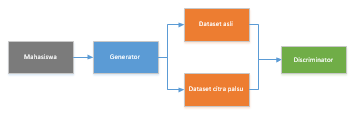
\includegraphics[width=4cm]{figures/1174054/8/1.png}
	\centering
	\caption{Generator}
\end{figure}

\item Jelaskan dengan ilustrasi gambar sendiri apa itu diskriminator dengan perumpamaan dosen anda sebagai diskriminatornya.\\
Diskriminator adalah mencoba untuk membedakan antara data nyata dan data yang dihasilkan oleh generator. Diskriminator mencoba memasukkan data yang masuk ke dalam kategori yang telah ditentukan. Sehingga dapat melakukan klasifikasi multi-kelas atau klasifikasi biner.
\begin{figure}[H]
	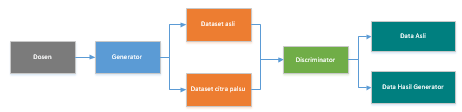
\includegraphics[width=4cm]{figures/1174054/8/2.png}
	\centering
	\caption{Diskriminator}
\end{figure}

\item Jelaskan dengan ilustrasi gambar sendiri bagaimana arsitektur generator dibuat.\\
Arsitektur generator dibuat bisa kita lihat pada gambar berikut :
\begin{figure}[H]
	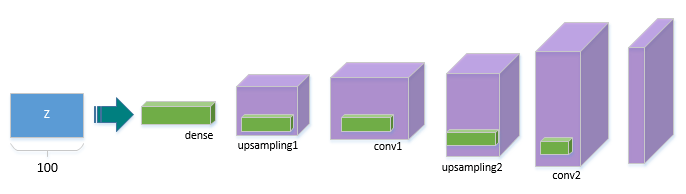
\includegraphics[width=4cm]{figures/1174054/8/3.png}
	\centering
	\caption{Arsitektur Generator}
\end{figure}

\item Jelaskan dengan ilustrasi gambar sendiri bagaimana arsitektur diskriminator dibuat.\\
Arsitektur diskriminator dibuat bisa kita lihat pada gambar berikut :
\begin{figure}[H]
	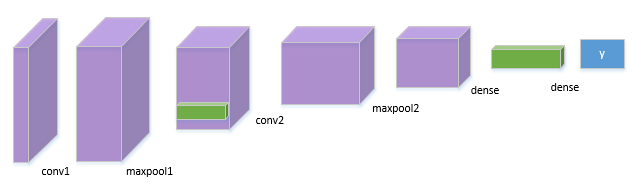
\includegraphics[width=4cm]{figures/1174054/8/4.png}
	\centering
	\caption{Arsitektur Diskriminator}
\end{figure}

\item Jelaskan dengan ilustrasi gambar apa itu latent space.\\
Latent space adalah representasi dari data yang terkompredi dimana titik data serupa lebih dekat bersama dalam ruang. Latent space berfungsi untuk mempelajari fitur data dan menemukan representasi data yang lebih sederhana untuk dianalisis.
Berikut adalah ilustrasi gambar latent space :
\begin{figure}[H]
	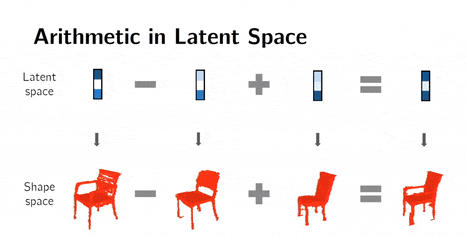
\includegraphics[width=4cm]{figures/1174054/8/5.png}
	\centering
	\caption{Latent Space}
\end{figure}

\item Jelaskan dengan ilustrasi gambar sendiri apa itu adversarial play.\\
Dalam GAN Adversial play adalah persaingan antara generator dan diskriminator. Untuk lebih jelasnya bisa dilihat pada gambar berikut :
\begin{figure}[H]
	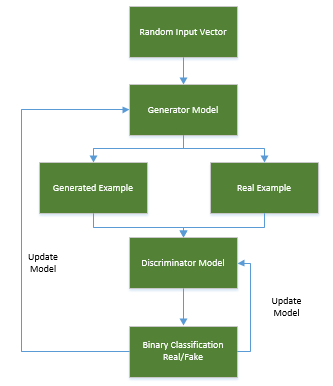
\includegraphics[width=4cm]{figures/1174054/8/6.png}
	\centering
	\caption{Adversial Play}
\end{figure}

\item Jelaskan dengan ilustrasi gambar apa itu Nash Equilibrium.\\
Nash equilibrium adalah suatu konsep dalam teori permainan dimana hasil optimal dari permainan adalah tidak ada insentif untuk menyimpang dari strategi awal. 
\begin{figure}[H]
	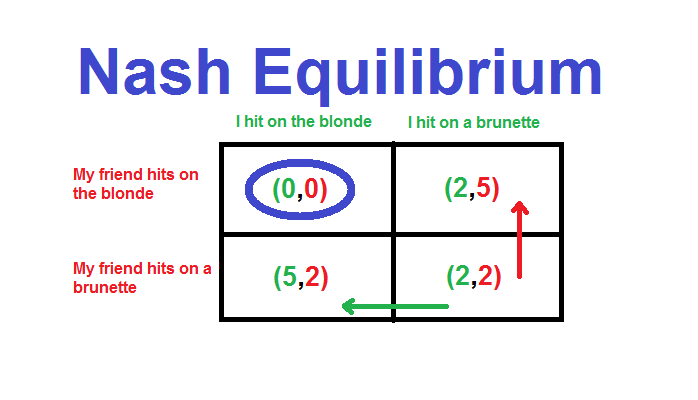
\includegraphics[width=4cm]{figures/1174054/8/7.png}
	\centering
	\caption{Nash Equilibrium}
\end{figure}

\item Sebutkan dan jelaskan contoh-contoh implementasi dari GAN.\\
Menurut saya, implementasi dari GAN yaitu MAPS dan IKEA, karena pada maps dan ikea sudah menerapkan bentuk 3 dimensi yang bisa lebih menarik perhatian pengguna. Selain itu, contoh implementasi dari GAN yaitu mengenerate wajah kelinci, kuda, dan lain sebagainya.

\item Berikan contoh dengan penjelasan kode program beserta gambar arsitektur untuk membuat generator (neural network) dengan sebuah input layer, tiga hidden layer(dense layer), dan satu output layer(reshape layer).\\
Berikut adalah kode program dalam membuat generator (neural network) :
\lstinputlisting[firstline=9, lastline=21]{src/1174054/8/teori.py}

\item Berikan contoh dengan ilustrasi dari arsitektur diskriminator dengan sebuah input layer, 3 buah hidden layer, dan satu output layer.\\
Berikut adalah kode program dalam membuat arsitektur diskriminator:
\lstinputlisting[firstline=24, lastline=36]{src/1174054/8/teori.py}

\item Jelaskan bagaimana kaitan output dan input antara generator dan diskriminator tersebut. Jelaskan kenapa inputan dan outputan seperti itu.\\
Gambar dari generator yang berhasil dideteksi oleh diskriminator sebagai gambar fake atau palsu, akan dikembalikan dengan feeback pakai generator, sehingga genearot bertugas untuk bisa membuat sekumpulan gambar palsu, yang nantinya dapat dilihat oleh diskriminator, sehingga diskriminator tidak bisa membedakan asli atau palsu.

\item Jelaskan apa perbedaan antara Kullback-Leibler di vergence (KL divergence)/relative entropy, Jensen-Shannon(JS) divergence /information radius (iRaD)/total divergence to the average dalam mengukut kualitas dari model.\\
Perbedaanya yaitu memiliki model dari rumus yang berbeda-beda sehingga dapat mempengaruhi hasil train dan test. Diantara keduanya yang paling terkenal adalah KL divergence, karena dia memiliki beberapa rumus yang bagus sedangkan JS tidak memilikinya.

\item Jelaskan apa itu fungsi objektif yang berfungsi untuk mengukur kesamaan antara gambar yang dibuat dengan yang asli.\\
Yaitu suatu ukuran yang penting untuk menilai kualitas suatu model, sehingga nantinya akan melihat keseimbangan di Nash.
fungsi objektif merupakan fungsi yang akan mengambil parameter data dan model sebagai argumen, dan dapat dievaluasi untuk mengembalikan angka sehingga mampu membedakan gambar yang asli dan yang di buat/fake.

\item Jelaskan apa itu scoring algoritma selain mean suare error atau cross entropy seperti the inception score dan the frechet inception distance.\\
The inception score adalah algoritma penilaian yang paling banyak digunakan untuk GAN. The Frechet Inception distance adalah suatu algoritma yang biasa digunakan Untuk mengatasi berbagai kekurangan Skor awal

\item Jelaskan kelebihan dan kekurangan GAN.\\
Kelebihan GAN yaitu GAN dapat memvisualisasikan bentuk model menjadi plot. Sedangkan untuk kekurangan GAN yaitu model susah untuk diimplementasikan sehingga membuat data training menjadi lemah.

\end{enumerate}

\subsection{Praktek}
\begin{enumerate}
\item Nomor 1\\
3D Convulations menerapkan filter 3 dimensi ke kumpulan data dan filter 3 arah yaitu x,y,dan z untuk menghitung representasi fitur tingkat rendah. Bentuk outputnya yaitu ruang volume 3 seperti kubus atau berbentuk kubus. 3D sangat membantu dalam mendeteksi peristiwa dalam video, gambar medis, dll. GAN adalah arsitektur jaringan saraf tiruan yang dimaksudkan untuk membuat data yang benar-benar baru, dari nol hingga tidak ada sama sekali, dimana dalam melihat target GAN adalah berupa data gambar. Singkatnya, jaringan GAN berfungsi untuk memberikan gambar baru berdasarkan koleksi gambar yang telah ada sebelumnya selama proses training.

\item Nomor 2\\
\hfill\break
	\lstinputlisting[firstline=32, lastline=62]{src/1174054/8/run.py}
Maksud dari kode diatas yaitu melakukan create generator yaitu gloss, dan bentuk jaringan generator dapat kita lihat berkebalikan dengan struktur jaringan saraf pada umumnya. Generator biasanya menerima input sebuah vektor z misalnya, yang kemudian akan diubah menjadi sebuah output 3D atau 3 dimensi. Selain itu, pada kode diatas terdiri dari 5 layer, yaitu satu input layer, tiga hidden layer, dan satu output layer.

\item Nomor 3\\
\hfill\break
	\lstinputlisting[firstline=67, lastline=105]{src/1174054/8/run.py}
Kode diatas merupakan diskriminator network. Jaringan Discriminator merupakan jaringan klasifikasi biner yang menerima input gambar tiga dimensi dan mengeluarkan klasifikasi menyatakan input gambar adalah gambar asli dari dataset atau merupakan gambar buatan Generator. Diskriminator dilatih dengan dataset yang diambil dari Generator, lalu di training untuk membedakan keduanya. Gambar dari Generator yang berhasil di deteksi oleh Diskriminator sebagai gambar fake, akan dikembalikan dengan feedback pke generator. Kini Generator bertugas untuk bisa membuat sekumpulan gambar palsu, yang nantinya dapat dilihat oleh Diskriminator, lalu, Diskriminator tidak bisa membedakan fake dan real.

\item Nomor 4\\
Proses Training 3D GAN yaitu :
\begin{itemize}
\item Terdapat sebuah vektor noise dengan dimensi 200 dari distribusi Gaussian (normal)
\item Mengenerate gambar palsu menggunakan model generator
\item Melatih jaringan generator dengan gambar yang asli (sampel dari data yang real) dan dengan gambar palsu yang dihasilkan oleh generator.
\item Gunakan adversial model untuk melatih generator model, jangan melatih diskriminator model
\item Ulangi langkah tersebut dengan jumlah epoch tertentu
\end{itemize}

\item Nomor 5\\
Sebelum melakukan tahapan persiapan data, ada beberpa hal yang harus diperhatikan seperti :
\begin{itemize}
\item Membaca buku panduan Generative-Adversial-Network yang ada di github
\item Mempersiapkan laptop/pc yang memiliki speck yang bagus
\item Mengclone github atau mendownload file yang dibutuhkan
\item Mendownload dataset yang digunakan
\item Membuat folder baru logs dan results
\end{itemize}

\item Nomor 6\\
Dataset yang digunakan 3DShapesNet yang disa didownload pada link yang sudah dibagikan. Dan untuk membuka data, kita hanya tinggal klik kanan file tersebut lalu pilih extract file, maka filenya akan terbuka. Sedangkan isi file tersebut ada beberapa folder. Dan diantara folder tersebut terdapat folder volumetric data yang didalamnya terdapat folder lagi yaitu folder train yang berisi train dan folder test yang berisi data testing

\item Nomor 7\\
Voxel atau Volume Pixel adalah suatu titik dalam ruang tiga dimensi. Suatu voxel mendefinisikan posisi dengan tiga koordinat dalam arah x,y, dan z. Suatu voxel merupakan unit dasar dalam mewakili gambar tiga dimensi, berikut adalah contoh ilustarasi atau penggambaran dari voxel
\begin{figure}[H]
	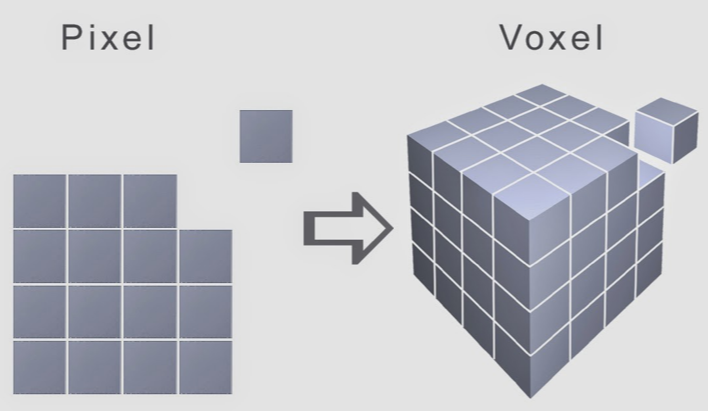
\includegraphics[width=4cm]{figures/1174054/8/8.png}
	\centering
	\caption{Voxel}
\end{figure}

\item Nomor 8\\
\hfill\break
	\lstinputlisting[firstline=9, lastline=25]{src/1174054/8/1174054.py}
Maksud dari kode diatas yaitu memvisualisasikan dataset dalam suatu tampilan plot, disini saya memiliki sofa. Untuk memvisualisasikan dataset tersebut, ada beberapa langkah yang harus dilakukan, yaitu mengimport library yang akan digunakan nantinya, meload data file .mat dan melalukan read memakai matplotlib. Maka kurang lebih hasilnya seperti gambar berikut :
\begin{figure}[H]
	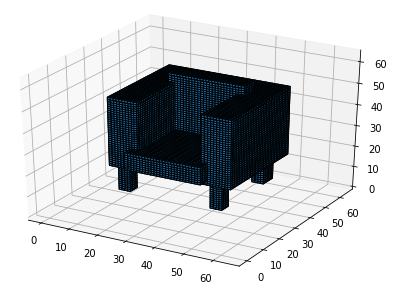
\includegraphics[width=4cm]{figures/1174054/8/9.png}
	\centering
	\caption{Hasil Nomor 8}
\end{figure}

\item Nomor 9\\
\hfill\break
	\lstinputlisting[firstline=32, lastline=62]{src/1174054/8/run.py}
Maksud dari kode diatas yaitu berfungsi untuk membuat generator dimana memiliki ketentuan gen sebagai variabel dan membuat fungsi atau variabel gen model kemudian dilalukan return.

\item Nomor 10\\
\hfill\break
	\lstinputlisting[firstline=67, lastline=105]{src/1174054/8/run.py}
Maksud dari kode diatas yaitu berfungsi untuk membangun suatu diskriminator yang dimana berfungsi untuk mendefinisikan seluruh gambar yang sudah diload generator sebagai gambar yang fake atau real.

\item Nomor 11\\
\hfill\break
	\lstinputlisting[firstline=158, lastline=160]{src/1174054/8/run.py}
Maksud dari kode program tersebut yaitu jika interpreter python menjalankan if name == main sebagai program utam, setelah itu, kita menetapkan variabel name untuk memiliki nilai main, lalu jika file tersebut sedang diimport dari modul lain, name akan ditetapkan sebagai nama modul. nama modul tersedia sebagai nilai untuk name variabel global.

\item Nomor 12\\
\hfill\break
	\lstinputlisting[firstline=163, lastline=172]{src/1174054/8/run.py}
Maksud dari kode diatas yaitu berfungsi untuk melakukan atau meload dataset dengan ketentuan data yang hanya dalam folder chair pada data train

\item Nomor 13\\
\hfill\break
	\lstinputlisting[firstline=176, lastline=185]{src/1174054/8/run.py}
Maksud dari kode diatas yaitu kita menggunakan Adam sebagai algoritma pengoptimalan dan binary crossentropy sebagai kerugian loss.

\item Nomor 14\\
\hfill\break
	\lstinputlisting[firstline=188, lastline=194]{src/1174054/8/run.py}
Maksud dari kode diatas yaitu kita memasukkan random vektor kedalam generator model lalu membagi dua yaitu generated example dan real example, dan untuk meneruskannya ke diskriminator model sebagai real atau fake

\item Nomor 15\\
\hfill\break
	\lstinputlisting[firstline=197, lastline=200]{src/1174054/8/run.py}
Maksud dari kode diatas yaitu berfungsi untuk melakukan load data pada dataset

\item Nomor 16\\
\hfill\break
	\lstinputlisting[firstline=203, lastline=205]{src/1174054/8/run.py}
Maksud dari kode diatas yaitu berfungsi untuk membuat tensorboard yang nantinya bisa diakses melaluo localhost

\item Nomor 17\\
\hfill\break
	\lstinputlisting[firstline=208, lastline=209]{src/1174054/8/run.py}
Maksud dari kode diatas yaitu berfungsi untuk melakukan reshape agar shape yang dihasilkan tidak terlalu besar, yaitu dengan membuat variabel real dan fake.

\item Nomor 18\\
\hfill\break
	\lstinputlisting[firstline=212, lastline=217]{src/1174054/8/run.py}
Maksud dari kode diatas yaitu berfungsi untuk melakukan training epoch, karena jika epoch semakin banyak maka kualitas training yang dihasilkan akan semakin baik.

\item Nomor 19\\
\hfill\break
	\lstinputlisting[firstline=220, lastline=223]{src/1174054/8/run.py}
Maksud dari kode diatas yaitu terdapat kata bach, yang artinya adalah jumlah file yang akan ditraining

\item Nomor 20\\
\hfill\break
	\lstinputlisting[firstline=226, lastline=227]{src/1174054/8/run.py}
Maksud dari kode diatas yaitu berfungsi untuk membuat gambar bersih dari noise dan juga mampu menyesuaikan shape

\item Nomor 21\\
\hfill\break
	\lstinputlisting[firstline=230, lastline=235]{src/1174054/8/run.py}
Maksud dari kode diatas yaitu berfungsi untuk membuat sample gambar palsu yang akan dikirimkan atau diteruskan ke diskriminator

\item Nomor 22\\
\hfill\break
	\lstinputlisting[firstline=238, lastline=247]{src/1174054/8/run.py}
Maksud dari kode diatas yaitu berfungsi untuk membuat diskriminator bisa load gambar fake dan real dari generator, oleh karena itu, ada generator loss dan diskriminator loss untuk melihat seberapa baik kualitas yang dihasilkan

\item Nomor 23\\
\hfill\break
	\lstinputlisting[firstline=250, lastline=259]{src/1174054/8/run.py}
Maksud dari kode diatas yaitu berfungsi untuk melakukan print gloss untuk generator dan juga dloss untuk diskriminator

\item Nomor 24\\
\hfill\break
	\lstinputlisting[firstline=262, lastline=270]{src/1174054/8/run.py}
Dari kode diatas, kita bisa melihat terdapat perulangan, maksudnya untuk melakukan perbandingan dari hasil yang sudah didapat

\item Nomor 25\\
\hfill\break
	\lstinputlisting[firstline=273, lastline=279]{src/1174054/8/run.py}
Dari kode diatas terdapat tensorboard yang merupakan sebuah aplikasi web localhost yang biasanya digunakan untuk memeriksa dan menyelesaikan grafik dari hasil tensorflow

\item Nomor 26\\
\hfill\break
	\lstinputlisting[firstline=282, lastline=283]{src/1174054/8/run.py}
Dalam kode diatas terdapat H5, H5 adalah suatu file yang merupakan file data yang disimpan dalam format data hirarki (HDF), yang berisi array multidimensi data ilmiah

\item Nomor 27\\
\hfill\break
	\lstinputlisting[firstline=286, lastline=303]{src/1174054/8/run.py}
Maksud dari kode diatas merupakan tahap akhir untuk melakukan testing dari model yang telah dibuat dan buat model dari yang sudah dicreate sebelumnya yaitu generator dan diskriminator,berikut adalah ilustrasi gambarnya :
\begin{figure}[H]
	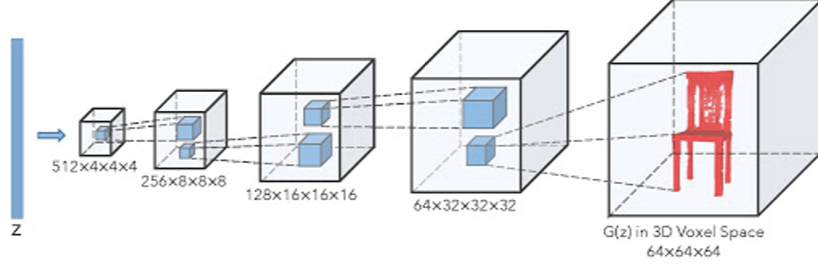
\includegraphics[width=4cm]{figures/1174054/8/10.png}
	\centering
	\caption{Hasil Nomor 27}
\end{figure}

\end{enumerate}

\subsection{Penanganan Error}
\begin{enumerate}
	\item File Not Found Error
	\begin{figure}[H]
		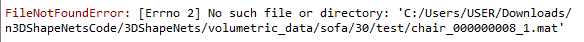
\includegraphics[width=4cm]{figures/1174054/8/error.png}
		\centering
		\caption{File Not FOund Error}
	\end{figure}

	\item Cara Penanganan Error
	\begin{itemize}
		\item File Not Found Error
		\hfill\break
		Error tersebut karena disebabkan gagal load dataset karena salah penamaan direktori.
	\end{itemize}
\end{enumerate}

\subsection{Bukti Tidak Plagiat}
\begin{figure}[H]
	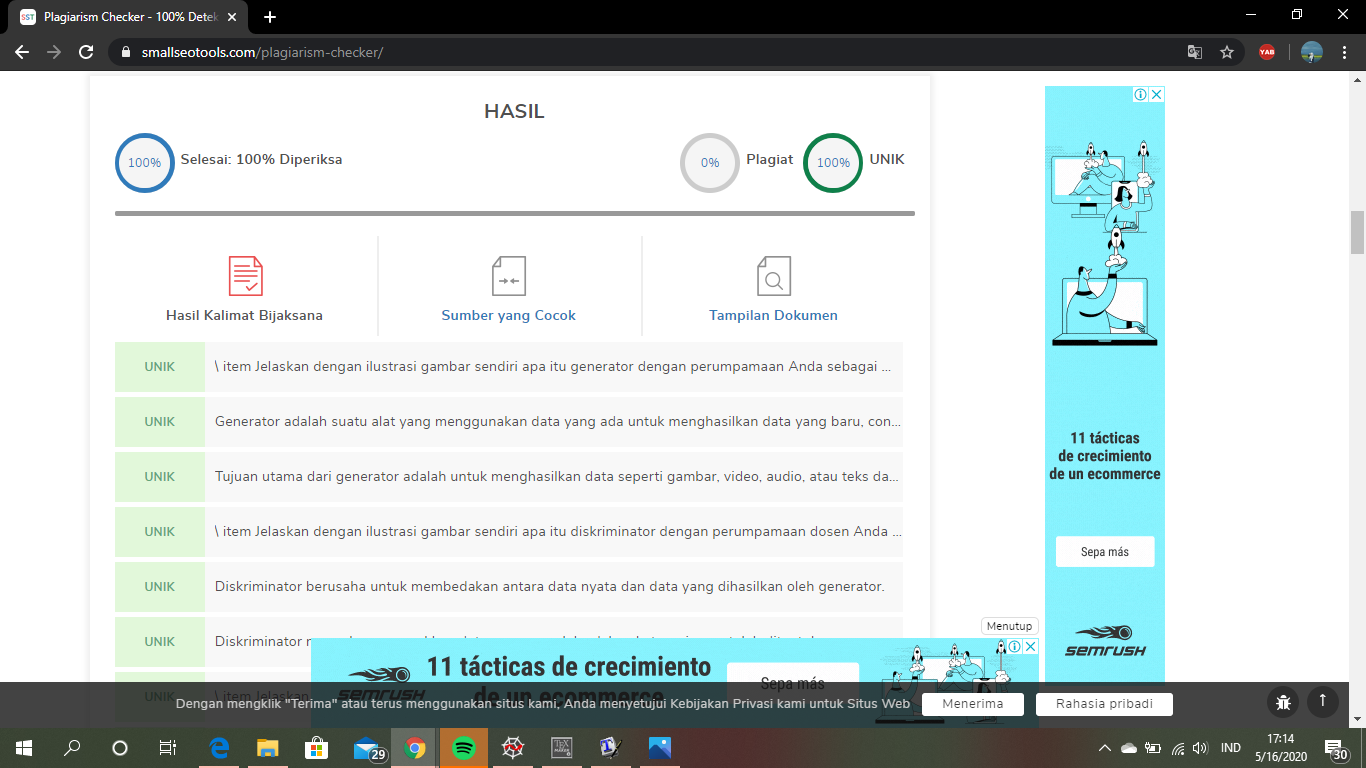
\includegraphics[width=4cm]{figures/1174054/8/plagiarisme.png}
	\centering
	\caption{Bukti Plagiarisme}
\end{figure}

\subsection{Link Youtube}